% This is samplepaper.tex, a sample chapter demonstrating the
% LLNCS macro package for Springer Computer Science proceedings;
% Version 2.21 of 2022/01/12
%
\documentclass[runningheads]{llncs}
%
\usepackage[T1]{fontenc}
% T1 fonts will be used to generate the final print and online PDFs,
% so please use T1 fonts in your manuscript whenever possible.
% Other font encondings may result in incorrect characters.
%
\usepackage{graphicx}

% Used for displaying a sample figure. If possible, figure files should
% be included in EPS format.
%
% If you use the hyperref package, please uncomment the following two lines
% to display URLs in blue roman font according to Springer's eBook style:
\usepackage{color}
%\renewcommand\UrlFont{\color{blue}\rmfamily}
%
\begin{document}
%
\title{A Comprehensive Survey of Arabic Large Language Models in Retrieval-Augmented Generation (RAG) Systems\thanks{Supported by organization x.}}
%
%\titlerunning{Abbreviated paper title}
% If the paper title is too long for the running head, you can set
% an abbreviated paper title here
%
\author{First Author\inst{1}\orcidID{0000-1111-2222-3333} \and
Second Author\inst{2,3}\orcidID{1111-2222-3333-4444} \and
Third Author\inst{3}\orcidID{2222--3333-4444-5555}}
%
\authorrunning{F. Author et al.}
% First names are abbreviated in the running head.
% If there are more than two authors, 'et al.' is used.
%
\institute{Princeton University, Princeton NJ 08544, USA \and
Springer Heidelberg, Tiergartenstr. 17, 69121 Heidelberg, Germany
\email{lncs@springer.com}\\
\url{http://www.springer.com/gp/computer-science/lncs} \and
ABC Institute, Rupert-Karls-University Heidelberg, Heidelberg, Germany\\
\email{\{abc,lncs\}@uni-heidelberg.de}}
%
\maketitle              % typeset the header of the contribution
%
\begin{abstract}
The abstract should briefly summarize the contents of the paper in
150--250 words.

\keywords{First keyword  \and Second keyword \and Another keyword.}
\end{abstract}
%
%
%
\section{Introduction}
Large Language Models (LLMs) have become foundational in Natural Language Processing (NLP),driving advancements in various AI applications.These models are pre-trained  on vast amounts of text data and then fine-tuned for specific tasks.Their success stems from their ability to act as implicit knowledge  bases\cite{ref_AlKhamissi2022},storing information learned during training within their parameters and generating responses by retrieving this stored knowledge.However, LLMs face significant limitations, particularly in domain-specific\cite{Singhal2023} or knowledge-intensive tasks\cite{ref_proc2}.One major issue is the hallucination\cite{Zhang2023} problem, where LLMs generate coherent and fluent but factually incorrect responses,To address these challenges, Retrieval-Augmented Generation (RAG)\cite{Lewis2020} has emerged as a powerful solution .

RAG enhances LLMs by integrating external knowledge databases, allowing the models to retrieve relevant information in real-time. This approach not only reduces hallucinations by grounding responses in factual data but also enables real-time updates without the need for retraining the model. As a result, RAG has become a key technology for improving the accuracy, reliability, and applicability of LLMs, particularly in specialized fields requiring factual precision.However,while RAG has been extensively explored and applied in English\cite{fan2024}, its potential remains largely untapped in other languages, especially Arabic. This gap is particularly striking given that Arabic is spoken by approximately 422 million people, making it one of the most widely used languages globally. 

Arabic remains underrepresented in the field of natural language processing, particularly in the context of RAG systems. The language's unique linguistic features and the diversity of its dialects \cite{Darwish2021}, which differ significantly from Modern Standard Arabic (MSA), add layers of complexity to text processing, retrieval, and generation. Addressing This research gap underscores the need to explore and adapt RAG methodologies specifically for Arabic, ensuring that its rich linguistic diversity is adequately addressed in modern NLP applications.

The architecture of a RAG system is built around several core components, with the retriever and generator playing the most critical roles.The retriever is responsible for fetching relevant text from an external knowledge base that serves as context for the generator.This context enables the generator to produce tailored, accurate responses by augmenting its pre-existing knowledge with the most current and domain-specific information available.If the retriever fails to provide relevant context, the entire system’s performance is compromised.To achieve effective retrieval, semantically rich embeddings are used to capture the meaning of text and identify the most relevant documents,
most state-of-the-art embedding models are trained on English data, raising questions about their ability to accurately capture the semantic nuances of Arabic .

Building on the challenges identified in Arabic retrieval,The generator synthesizes the retrieved information into a coherent and contextually accurate response, a process that becomes even more demanding when handling the nuances of Arabic. However, Arabic generation faces its own hurdles—complex morphology, dialectal diversity, and limited training data often lead to inconsistencies.To our knowledge, this survey is the first to comprehensively review Arabic AI applications in both retrieval and generation within RAG systems, identifying key gaps and paving the way for future improvements in Arabic NLP.

\section{Related works}
In recent years, extensive research has focused on Arabic language models and their applicability in a variety of NLP tasks. But as the subject develops, it is essential to examine the major findings from various surveys in order to comprehend the state of Arabic natural language processing and the challenges it faces. These surveys cover a wide range of subjects, including evaluation techniques, domain-specific applications, model structures, and dataset resources. In contrast to multilingual and general-purpose approaches, this section attempts to give a summary of the most relevant surveys, categorized into groups, that address unique challenges of Arabic language models. \newline
\textbf{1.Arabic Model Architectures }\\
The body of research on large language models has grown rapidly, with several surveys addressing both multilingual models and Arabic-specific challenges. For example, "A Survey of Large Language Models for Arabic Language and its Dialects"\cite{ref_proc10} not only reviews various Arabic LLM architectures and the diverse datasets (Classical Arabic (CA), Modern Standard Arabic (MSA), and Dialectal Arabic (DA)) used for pretraining but also places a strong emphasis on openness. It evaluates the availability of source code, training data, model weights, and documentation—a key factor for reproducibility and further development in Arabic NLP. Through these objectives, the survey offers a comprehensive resource that maps the current landscape of Arabic LLMs and outlines clear directions for future advancements\newline
\textbf{2.Advances in Multilingual LLMs}\\
Building on these insights into Arabic language models and their openness, it's important to broaden the perspective to include recent advancements in multilingual LLMs. In particular Multilingual LLMs: A Systematic Survey\cite{Zhu2024} reviews architectural innovations, multilingual dataset construction, and evaluation frameworks for cross-lingual knowledge, reasoning, and safety. Collectively, these works emphasize advancements in addressing linguistic disparities, improving model robustness, and advancing real-world applications, while underscoring unresolved challenges like resource fairness and equitable performance across languages. A Survey of Multilingual Large Language Models\cite{ref_proc11} introduces a taxonomy for alignment strategies (parameter-tuning PTA vs. parameter-frozen alignment FTA),catalogs data resources, and highlights challenges in low-resource language support.Finally,A Survey on Multilingual Large Language Models:Corpora, Alignment, and Bias \cite{ref_proc12}examines multilingual LLMs by analyzing language imbalance and cross-lingual transfer capabilities, while reviewing the diverse datasets and corpora used for model training. Additionally, it explores whether current models can achieve a universal language representation and addresses inherent biases by summarizing debiasing strategies and bias evaluation datasets .\\
\textbf{3.Resource and Data Surveys} \\
In A Panoramic Survey of Natural Language Processing in the Arab World,\cite{Darwish2021} Describe Arabic natural language processing, emphasizing the limited availability variety of corpora. They highlight key challenges such as dialectal diversity and data scarcity, which significantly impact the development and performance of NLP systems in the Arab world.
Building on the challenges identified in Arabic NLP Ghaddar et al. (2022) delve deeper into the quality and scale of Arabic pre-training datasets in their work, "Revisiting Pre-trained Language Models and their Evaluation for Arabic Natural Language Understanding."\cite{ref_proc15} This study systematically evaluates existing Arabic PLMs, uncovering significant resource gaps and emphasizing how improved data quality and scalability might enhance performance on a variety of NLP applications. Their insights offer a clear roadmap for improving evaluation practices and optimizing Arabic language models,thereby resolving some of the critical problems highlighted in previous surveys. . \newline
\textbf{4.Application-Specific Surveys} \newline
In the field of Arabic language modeling, various surveys have concentrated on specific NLP applications. In "A Survey on Arabic Named Entity Recognition: Past, Recent Advances, and Future Trends," \cite{qu2023}This survey provides the first comprehensive analysis of Arabic Named Entity Recognition (NER), covering resources, methodologies (rule-based, machine/deep learning, pre-trained models), and recent advancements. It systematically benchmarks existing approaches on ANERCorp and AQMAR datasets under standardized splits to enable fair comparisons, addressing inconsistencies in prior evaluations.it serves as a foundational guide for advancing Arabic NER development.For Text Summarization the survey "Deep Transformer Language Models for Arabic Text Summarization: A Comparison Study"\cite{couikhi2022}fills a critical gap in Arabic abstractive text summarization (ATS) research by offering a comprehensive comparison of transformer-based Arabic and Arabic-supported multilingual ATS systems. It evaluates multiple models using a range of metrics and diverse datasets—including Arabic Headline Summaries (AHS) and Arabic News Articles (ANA)—and investigates the impact of fine-tuning on summary quality. Through empirical analysis of both transformer language models and deep-learning-based ATS approaches, the study provides detailed insights into the strengths and limitations of current systems, paving the way for future advancements.
\begin{table}
	\caption { Arabic AI Models Studies in Retrieval-Augmented Generation (RAG)  }\label{tab:arabic_rag}
	\centering
	\resizebox{\textwidth}{!}{ 
		\begin{tabular}{|p{3.5cm}|p{1.4cm}|p{3.5cm}|p{4.5cm}|p{3cm}|p{3.5cm}|p{3.5cm}|}
		\hline
		\multicolumn{7}{|c|}{\textbf{Studies on Retrieval-Only Models}} \\
		\hline
			\textbf{Paper} & \textbf{year} &
		    \textbf{Retrieval Component Studied} 	& 
		    \textbf{Arabic Model Name} & \textbf{Datasets Used} & \textbf{Evaluation Metrics} & \textbf{Challenges}  \\
			\hline
			Semantic Embeddings for Arabic Retrieval
			Augmented Generation (ARAG) \cite{ref_arag2023} & 2023 &\textbf{Retrieval} :Semantic   Embeddings &
			Microsoft(e5s,e5b,e5l)\newline DistillBert(hf1,hf2),\newline Openai  Ada embedding \newline  Cohere Multilingual Embedding \newline Meta SONAR  \newline Google LaBSE\newline mpnet-base-v2   & Arabic Reading Comprehension Dataset (ARCD) & Recall@k.&-Embedding Size Constraints \newline      -Need for Language Specific Evaluation Metrics \\
			\hline
			Evaluation of Semantic Search and its Role in Retrieved for Arabic Language\cite{Mahboub2024} & 2024 &\textbf{Retrieval} :Semantic search in Arabic &Encoder 1: MiniLM \newline
			Encoder 2: CMLM\newline
			Encoder 3: MPNet \newline
		    Encoder 4: DistilBERT\newline
		    Encoder 5 : XLM RoBERTa &FAQs: 816 questions with verifiable answers & NDCG@3 \newline MRR@3 \newline mAP@3 & -Embedding size constraints. \newline -Arabic complexity \\
			\hline
			Arabic RAG Leaderboard: A Comprehensive Framework for Evaluating Arabic Language Retrieval Systems\cite{ref_TARL2025} & 2025&
			\textbf{Retrieval}: Semantic Embedding . \newline 
			\textbf{Reranking}:Refine retrieved documents & Retrieval :GATE-AraBERT-v1 \newline
			Reranking : ARA-Reranker-V1\newline
			 &Retrieval:"Web Search Dataset" \newline Reranking:sourced from TyDi QA and MKQA datasets & NDCG \newline MRR \newline mAP \newline Recall@k &  Arabic’s morphological complexity \newline  Dialect diversity\\
			\hline
	        \multicolumn{7}{|c|}{\textbf{Studies on Both Retrieval and Generation}} \\
	        \hline
	       
	        \textbf{Paper} & \textbf{Year} & \textbf{RAG Component Studied} & \textbf{Arbic  Model Name} & \textbf{Datasets Used} & \textbf{Evaluation Metricsl} & \textbf{Chalenges} \\
	        \hline
			Exploring Retrieval Augmented Generation in Arabic \cite{ref_elbeltagy2024} & 2024 . &  \textbf{Retrieval}: Semantic Embedding \newline \textbf{Generation} : generate Arabic response  & \textbf{Retrieval}: AraVec , AraBERT ,OpenAI ,Cohere, Microsoft’s E5,  Ollama ,JAIS,BGE \newline \textbf{Generator}:GPT3.5, urbo, Mistral 
			7B, Llama 3, Mixtral, and JAIS.
			  & Ar-EduText dataset \newline ARCD dataset 
			  &\textbf{Retrival}:Recall@K (k=1,k=3,k=5) \newline \textbf{Generator}: F1 Score Bleu Score Cosine SimilarityR&-Lack of Detailed Metrics \newline -Dialect Diversity \\
			\hline
		Evaluating RAG Pipelines for Arabic Lexical Information Retrieval: A Comparative Study of Embedding and Generation Models\cite{ref_alrasheed2025} & 2025 & \textbf{Retrieval}: Word Embeddings , Sentence Embeddings \newline \textbf{Generator} : generatte Arabic lexical information&\textbf{Retrival}:CAMeLBERT, AraBERT-v2, E5-large Arabic-NLI ,AraELECTRA  \newline \textbf{Generator}: GPT-4o, Gemini-1.5-flash, SILMA-9B-Instruct, Aya8B GPT-3.5, AceGPT13B&Riyadh dictionary (88,000+ words)&\textbf{Retrival} Top-k Recall (k = 1, 3, 5) and MRR \newline \textbf{Generator}:F1-score(F1),
		Accuracy (Acc), and CosineSimilarity(Cos). &-handling of dialectal variations in queries and documents. \newline -Disparity in performance between sentence embeddings and word \\
			\hline
		Towards a Fully Arabic Retrieval-Augmented Generation (RAG) Pipeline\cite{nacer2024} & 2024 &\textbf{Retriever} (Embedding-based Retrieval with Semantic Chunking) \newline\textbf{ Reranker} (CrossEncoder-based Reranking) \newline \textbf{Generator} (Arabic Text Generation) & \textbf{Retriever} : GATE-AraBERT-v1 \newline \textbf{ Reranker}:ARA-Reranker-V1 (ARM-V1) \newline \textbf{Generator} : GPT-4 mini &Custom Arabic text corpus& Qualitative evaluation of contextual accuracy and clarity& Capturing Arabic semantic nuances and managing dialectal variations \\ \hline
	
		\end{tabular}
	} % End resizebox
\end{table}















%\subsection{A Subsection Sample}


%\subsubsection{Sample Heading} Only two levels of

%\paragraph{Sample Heading (Fourth Level)}







%\begin{figure}
%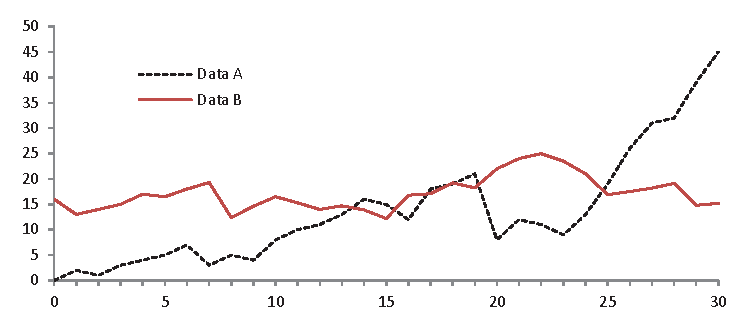
\includegraphics[width=\textwidth]{fig1.eps}
%\caption{A figure caption is always placed below the illustration.
%Please note that short captions are centered, while long ones are
%justified by the macro package automatically.} \label{fig1}
%\end{figure}%



% the environments 'definition', 'lemma', 'proposition', 'corollary',
% 'remark', and 'example' are defined in the LLNCS documentclass as well.
%

%For citations of references, we prefer the use of square brackets
%and consecutive numbers. Citations using labels or the author/year
%convention are also acceptable. The following bibliography provides
%a sample reference list with entries for journal
%articles~\cite{ref_article1}, an LNCS chapter~\cite{ref_lncs1}, a
%book~\cite{ref_book1}, proceedings without editors~\cite{ref_proc1},
%and a homepage~\cite{ref_url1}. Multiple citations are grouped
%\cite{ref_article1,ref_lncs1,ref_book1},
%\cite{ref_article1,ref_book1,ref_proc1,ref_url1}.

%\subsubsection{Acknowledgements} Please place your acknowledgments at
%the end of the paper, preceded by an unnumbered run-in heading (i.e.
%3rd-level heading).

%
% ---- Bibliography ----
%
% BibTeX users should specify bibliography style 'splncs04'.
% References will then be sorted and formatted in the correct style.
%
% \bibliographystyle{splncs04}
% \bibliography{mybibliography}
%
\newpage
\begin{thebibliography}{8}
\bibitem{ref_arag2023}
Abdelazim, H., Mohamed, A., Tharwat, M.: Semantic Embeddings for Arabic Retrieval Augmented Generation (ARAG). International Journal of Advanced Computer Science and Applications \textbf{14}(11), xx--yy (2023)


\bibitem{Mahboub2024}
Mahboub, A., Za’ter, M. E., Al-Rfooh, B., Estaitia, Y., Jaljuli, A., Hakouz, A.:  
Evaluation of Semantic Search and its Role in Retrieved-Augmented-Generation (RAG) for Arabic Language.  
In: arXiv preprint, arXiv:2403.18350v2, May 2024. Available at: \url{https://arxiv.org/abs/2403.18350}

\bibitem{ref_TARL2025}
Rashad, M.A., Shahid, H.: The Arabic RAG Leaderboard. \textit{Navid-AI} (2025). Available online at: \url{https://huggingface.co/spaces/Navid-AI/The-Arabic-Rag-Leaderboard}.


\bibitem{ref_elbeltagy2024}
El-Beltagy, S.R., Abdallah, M.A.: Exploring Retrieval Augmented Generation in Arabic. Procedia Computer Science, \textbf{00}, 000--000 (2024). Available online at: \url{www.sciencedirect.com}.

\bibitem{ref_alrasheed2025}
Al-Rasheed, R., Al Muaddi, A., Aljasim, H., Al-Matham, R., Alhoshan, M., Al Wazrah, A., AlOsaimy, A.:  
Evaluating RAG Pipelines for Arabic Lexical Information Retrieval: A Comparative Study of Embedding and Generation Models.  
In: El-Haj, M. (ed.), Proc. 1st Workshop on NLP for Languages Using Arabic Script, pp. 155--164.  
Association for Computational Linguistics, Abu Dhabi, UAE (2025).  
Available: \url{https://aclanthology.org/2025.abjadnlp-1.16/}  


\bibitem{ref_AlKhamissi2022}
AlKhamissi, B., Li, M., Celikyilmaz, A., Diab, M., Ghazvininejad, M.: A Review on Language Models as Knowledge Bases. In: arXiv preprint arXiv:2204.06031 (2022)


\bibitem{ref_proc2}
Kandpal, N., Deng, H., Roberts, A., Wallace, E., Raffel, C.: Large language models struggle to learn long-tail knowledge. In: International Conference on Machine Learning, pp. 15696--15707. PMLR (2023)

\bibitem{Zhang2023}
Zhang, Y., Li, Y., Cui, L., Cai, D., Liu, L., Fu, T., Huang, X., Zhao, E., Zhang, Y., Chen, Y., et al.: Siren’s song in the AI ocean: A survey on hallucination in large language models. In: arXiv preprint arXiv:2309.01219 (2023)


\bibitem{Singhal2023}
Singhal, K., Tu, T., Gottweis, J., Sayres, R., Wulczyn, E., Hou, L., Clark, K., Pfohl, S., Cole-Lewis, H., Neal, D., et al.: Towards expert-level medical question answering with large language models. In: arXiv preprint arXiv:2305.09617 (2023)


\bibitem{Lewis2020}
Lewis, P. S. H., Perez, E., Piktus, A., Petroni, F., Karpukhin, V., Goyal, N., Küttler, H., Lewis, M., Yih, W.-T., Rocktäschel, T., Riedel, S., Kiela, D.: Retrieval-Augmented Generation for Knowledge-Intensive NLP Tasks. In: NeurIPS, (2020)

\bibitem{fan2024}
Fan, W., Ding, Y., Ning, L., Wang, S., Li, H., Yin, D., Chua, T.-S., Li, Q.: A Survey on RAG Meeting LLMs: Towards Retrieval-Augmented Large Language Models. In: arXiv preprint arXiv:2405.06211 (2024)


\bibitem{Darwish2021}
Darwish, K., Habash, N., Abbas, M., Al-Khalifa, H., Al-Natsheh, H. T., Bouamor, H., Bouzoubaa, K., Cavalli-Sforza, V., El-Beltagy, S. R., et al.: A panoramic survey of natural language processing in the Arab world. In: Communications of the ACM, vol. 64, pp. 72--81. ACM, New York, NY, USA (2021)

\bibitem{nacer2024}
Nacar, O.: Towards a Fully Arabic Retrieval-Augmented Generation (RAG) Pipeline. In: --, (2024)


\bibitem{ref_proc10}
Mashaabi, M., Al-Khalifa, S., Al-Khalifa, H.: A Survey of Large Language Models for Arabic Language and its Dialects. In: arXiv preprint arXiv:2410.20238 (2024)

\bibitem{Zhu2024}
Zhu, S., Supryadi, Xu, S., Sun, H., Pan, L., Cui, M., Du, J., Jin, R., Branco, A., Xiong, D.: Multilingual Large Language Models: A Systematic Survey. In: arXiv preprint arXiv:2411.11072 (2024)

\bibitem{ref_proc11}
Qin, L., Chen, Q., Zhou, Y., Chen, Z., Li, Y., Liao, L., Li, M., Che, W., Yu, P. S.: A survey of multilingual large language models. In: Patterns, vol. 6, no. 1. Elsevier (2025). https://doi.org/10.1016/j.patter.2024.101118
 
\bibitem{ref_proc12}
Xu, Y., Hu, L., Zhao, J., Qiu, Z., Xu, K., Ye, Y., Gu, H.: A Survey on Multilingual Large Language Models: Corpora, Alignment, and Bias. In: arXiv preprint arXiv:2404.00929 (2024)

\bibitem{ref_proc15}
Ghaddar, A., Wu, Y., Bagga, S., Rashid, A., Bibi, K., Rezagholizadeh, M., Xing, C., Wang, Y., Xinyu, D., Wang, Z., Huai, B., Jiang, X., Liu, Q., Langlais, P.: Revisiting Pre-trained Language Models and their Evaluation for Arabic Natural Language Understanding. In: arXiv preprint arXiv:2205.10687 (2022)

\bibitem{qu2023}
Qu, X., Gu, Y., Xia, Q., Li, Z., Wang, Z., Huai, B.: A Survey on Arabic Named Entity Recognition: Past, Recent Advances, and Future Trends. In: arXiv preprint arXiv:2302.03512 (2023)

\bibitem{couikhi2022}
Chouikhi, H., Alsuhaibani, M.: Deep Transformer Language Models for Arabic Text Summarization: A Comparison Study. In: Applied Sciences, vol. 12, no. 23, article 11944. MDPI (2022). https://doi.org/10.3390/app122311944


\end{thebibliography}
\end{document}
